\chapter{Versuch 4: Widerstandsmessung mittels Vierdrahtmethode}

\section{Versuchsdurchführung}

\subsection{Versuchsaufbau}

\begin{figure}[H]
	\centering
	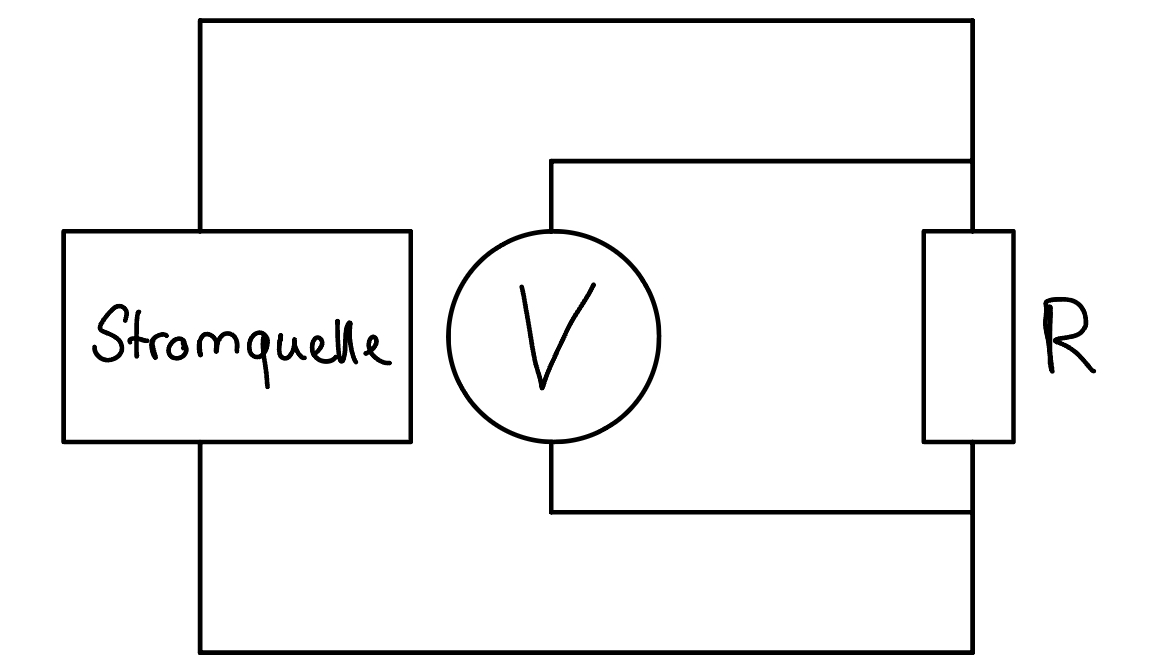
\includegraphics[height=7cm]{images/Versuch4/Schaltskizze.jpeg}
	\caption{Schaltungsskizze}
	\label{fig: Schaltungsskizze}
\end{figure}

\begin{figure}[H]
	\centering
	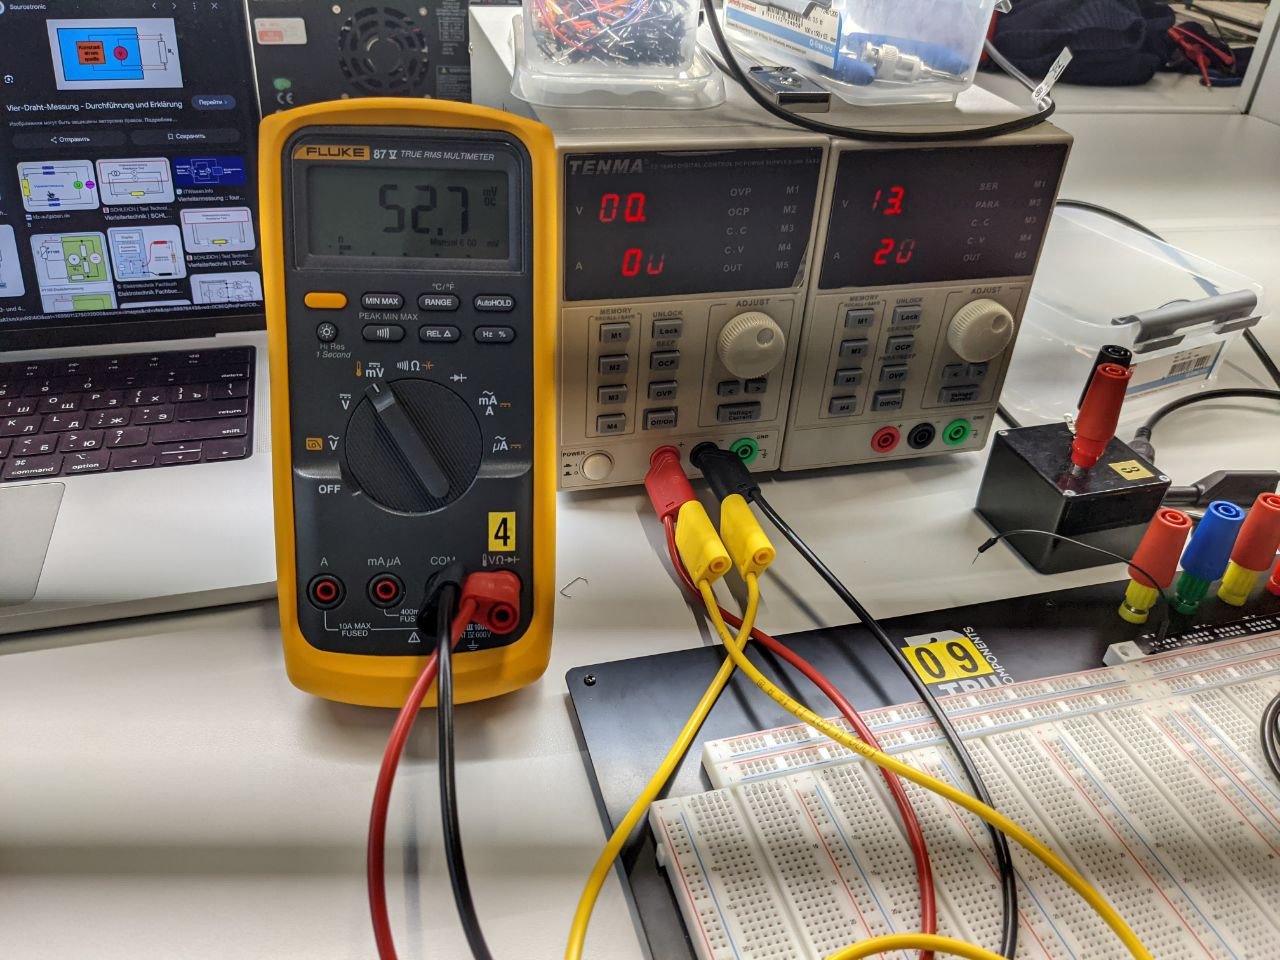
\includegraphics[height=7cm]{images/Versuch4/Versuchsaufbau.jpeg}
	\caption{Schaltungsskizze}
	\label{fig: Schaltungsskizze}
\end{figure}


Durch diesen Aufbau kann man am Voltmeter, bzw. dem Digital-Multimeter,
den Widerstand R errechnen. Dieser berechnet sich nach folgender Formel:

\begin{equation}
    R = \frac{U}{I}
    \label{eq:R}
\end{equation}

\subsection{Messung}
\label{subsec:Messung}
Durch das Verwenden einer Konstantstromquelle wird der Strom I konstant
auf 2,00A gehalten. Nun können wir die Spannung Messen. Diese beträgt
52,7 mV. Mit der Formel \ref*{eq:R} können wir nun den Widerstand
berechnen. Dieser beträgt 26,35m$\Omega$.

\section{Zusatzfragen}

Wie bereits in \ref{subsec:Messung} erwähnt, wird der Strom I konstant
gehalten. Dies bedeutet, dass es sich um eine Konstantstromquelle handelt.
Durch einen konstanten Wiederstand R würde eine Erhöhung des Stroms I
eine Erhöhung der Spannung U bedeuten. 
Grenzen dieses Strom liegen in der maximalen Belastbarkeit des Wiederstands
und der Konstantstromquelle. Die Konstantstromquelle darf nicht überlastet
werden, da sonst die Messung verfälscht wird. Allerdings sollte auch kein 
zu greinger Strom verwendet werden, da eine zu geringe Spannung auch zu
Verfälschungen, bzw. Ungenauigkeiten führen kann.

